\begin{tikzpicture}
\begin{scope}
\clip (1.175,1.1) rectangle (7.7,7.4) ;
\node[anchor=south west,inner sep=0] at (0,0) {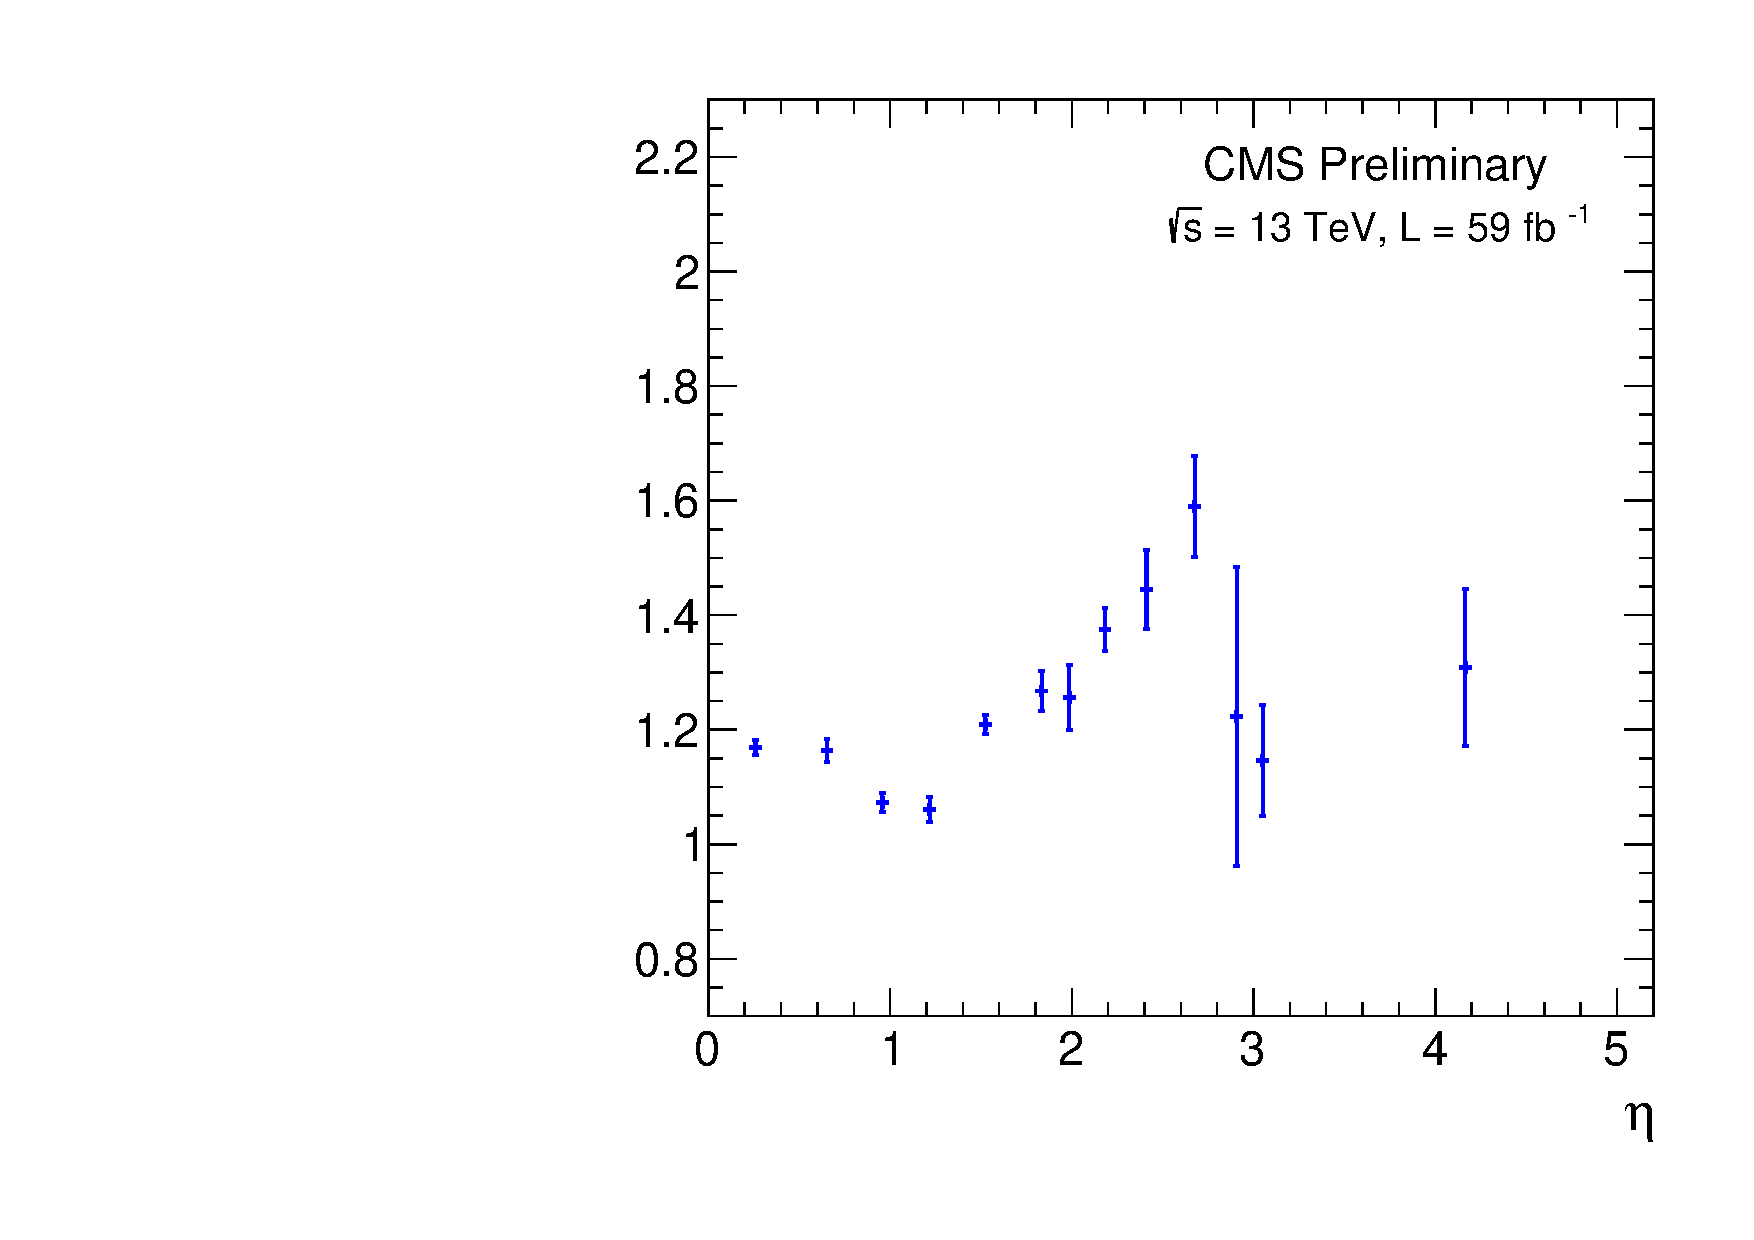
\includegraphics[width=8cm]{\PhDthesisdir/plots_and_images/my_plots/JERC/JER/Run2018ABCD/alpha_0_3/fine_eta_binning_Scale_factor_res_vs_ETA.pdf}};
\end{scope}

% above txt
\draw (7.7, 7.6) node [left] {\footnotesize Run 2018 ABCD, \SI{59}{\femto\barn^{-1}} (\SI{13}{\TeV})};

% masks
\fill [white] (4.2,6.3) rectangle (7.3,7.12);

% X axis
\foreach \val in {0,1,...,5}{
\draw ({1.2+(7.36-1.2)*\val/5}, .95) node {\small \val};
}
\draw (7.5, .5) node {\normalsize $\abs{\eta}$};

% Y axis
\foreach \val in {0.8,1.0,1.2,1.4,1.6,1.8,2.0,2.2}{
\draw (1.3, {1.55+(\val-0.8)/(2.2-0.8)*(6.975-1.55)}) node [left] {\small $\num{\val}$};
}
\draw (.25, 7.25) node [left, rotate=90] {JER SF};

% CMS disclaimer
\draw (1.1, 7.6) node [right] {\footnotesize CMS Data};
\draw (1.4, 6.8) node [right] {\OwnWork};
\end{tikzpicture}
